\sectionquestion{Removed Questions}

\begin{parts}

\part[1] \textbf{Select all that apply:} What characteristics apply to positional embeddings in Transformers?
    {%
    \checkboxchar{$\Box$} \checkedchar{$\blacksquare$} % change checkbox style locally
    \begin{checkboxes}
     \choice They enable the model to utilize the order of the sequence in making predictions.
     \choice They can be either be learned during training or fixed using a predefined sinusoidal function.
     \choice They help the model maintain time-sensitive dependencies in data.
     \choice They are not effective in models with a single attention head.
     \choice None of the above
    \end{checkboxes}
    }
    \begin{soln}
    A, B, C
    \end{soln}
    \begin{qauthor}
    Kushagra Agarwal, Justify the use of positional embeddings in transformers.
    \end{qauthor}

\part Consider we use a self-attention block with queries $(Q)$ and keys $(K)$ of dimension $d_k$ and values $(V)$ of dimension $d_v$. Recall, that the self-attention computation is as follows:

\[ Attention(Q, K, V) = softmax(\frac{QK^T}{scaling factor}) V \]

Now, answer the following questions as they pertain to the self-attention mechanism used in transformers. 
    \begin{subparts}
    
        \subpart[2]  \textbf{Select all that apply:} Why is scaling the dot products necessary in the attention calculation?
   {%
    \checkboxchar{$\Box$} \checkedchar{$\blacksquare$} % change checkbox style locally
    \begin{checkboxes}
     \choice The scale of the dot product increases as the dimensions grow larger.
     \choice The gradients of the softmax function become extremely small.
     \choice For higher dimensions, the queries and keys dominate over the values in the attention calculation.
    \end{checkboxes}
    }
        \begin{soln} 
            A, B. For large values of
$d_k$, the dot products grow large in magnitude, pushing the softmax function into regions where it has
extremely small gradients.
        \end{soln}

        \subpart[1]  \textbf{Select one:} What is the scaling factor used for the dot product of Q and K?:
    \begin{checkboxes}
        \choice $\frac{1}{d_k}$ 
        \choice $\frac{1}{\sqrt{d_k}}$ 
        \choice $\frac{1}{d_v}$ 
        \choice $\frac{1}{\sqrt{d_v}}$ 
    \end{checkboxes}
        \begin{soln} 
            B. We scale the dot products by $\frac{1}{\sqrt{d_k}}$.
        \end{soln}


        \subpart[2]  \textbf{Select one:} Now suppose we use eight attention heads $(h = 8)$ and enforce that all sublayers of the transformer produce outputs of dimension $d_{model} = 512$. Here, $d_k = d_v = d_{model} / h = 64$. What is the effect on computational cost in comparison to using single-headed attention with the same dimensions ($d_{model} = 512)$? :
    \begin{checkboxes}
        \choice No effect on computational cost, it will run in similar time as single-headed attention.
        \choice It scales linearly and using 8 attention heads will result in it running 8 times slower than single-headed attention.
        \choice It scales quadratically and using 8 attention heads will result in it running 64 times slower than single-headed attention.
    \end{checkboxes}
        \begin{soln} 
            A. Due to the reduced dimension of each head, the total computational cost
is similar to that of single-head attention with full dimensionality.
        \end{soln}

        \subpart[2]  \textbf{Select one:} The transformer encoder block has N layers, each with two sub-layers: A multi-headed self-attention block and a fully connected feed-forward network. To simplify, assume that the input to a sub-layer is x and its output is Sublayer(x). How are residual connections and Layer Normalization implemented in transformers?:
    \begin{checkboxes}
        \choice x + LayerNorm(Sublayer(x))
        \choice LayerNorm(x) + Sublayer(x)
        \choice LayerNorm(x + Sublayer(x)) 
    \end{checkboxes}
        \begin{soln} 
            C. LayerNorm(x + Sublayer(x))
        \end{soln}
        

    \end{subparts}
    \begin{qauthor}
        Aadit
    \end{qauthor}

\part[2] Markov decides that he is tired of ReLU, and decides to swap it out for softmax. Is this a good decision? Why or why not? % Describe the purpose of both ReLU and softmax in a CNN 
    \begin{soln}
    TODO
    \end{soln}
    \begin{qauthor}
    Erin?, Implement the common layers found in Convolutional Neural Networks (CNNs) such as linear layers, convolution layers, max-pooling layers, and rectified linear units (ReLU)
    \end{qauthor}


\part[1] \textbf{Select one:} We can perform the following tasks using a CNN:
    \begin{checkboxes}
        \choice upsampling with a stride $<1$ and downsampling with a stride $>1$
        \choice downsampling with a stride $<1$ and upsampling with a stride $>1$
        \choice only upsampling with a stride $<1$
        \choice only downsampling with a stride $<1$
    \end{checkboxes}
    \begin{soln}
        A
    \end{soln}
    \begin{qauthor}
        Annie
    \end{qauthor}

\part[2] \textbf{True or False:} In backpropagation, if the activation function used at a neuron is the ReLU (Rectified Linear Unit) function, then the derivative of the loss function with respect to the input of that neuron is always non-negative. Explain your reasoning below.
    \begin{checkboxes}
     \choice True 
     \choice False
    \end{checkboxes}
    \noindent\rule{\textwidth}{0.4pt} % First line for writing
    \noindent\rule{\textwidth}{0.4pt} % Second line for writing
    \begin{soln}
    False. The derivative of ReLU itself is 1 for \( x > 0 \) and 0 for \( x < 0 \). The derivative is undefined at \( x = 0 \), but is often considered 0 in implementations.

    When performing backpropagation, the gradient of the loss with respect to the input of a neuron using ReLU is computed by multiplying the derivative of the loss with respect to the output of the neuron (post-activation) by the derivative of the ReLU function. If the derivative of the loss with respect to the output is negative and the ReLU derivative is 1 (for \( x > 0 \)), the resulting gradient with respect to the input will also be negative. 
    \end{soln}

    \begin{qauthor}
    Monica, Describe the backpropagation algorithm for a CNN
    \end{qauthor}


\part[2] \textbf{Drawing:} Given the three binary classifiers $h_1, h_2, h_3$ with arrows indicating where they classify $y=+1$, what is the decision boundary of the weighted majority vote classifier if $h_2$ has twice the weight of $h_1$ and $h_3$? (For full credit, shade the region that is classified as $y=+1$. Assume that $\text{sign}(0) = +1$ when computing the weighted vote.)
    \begin{center}
    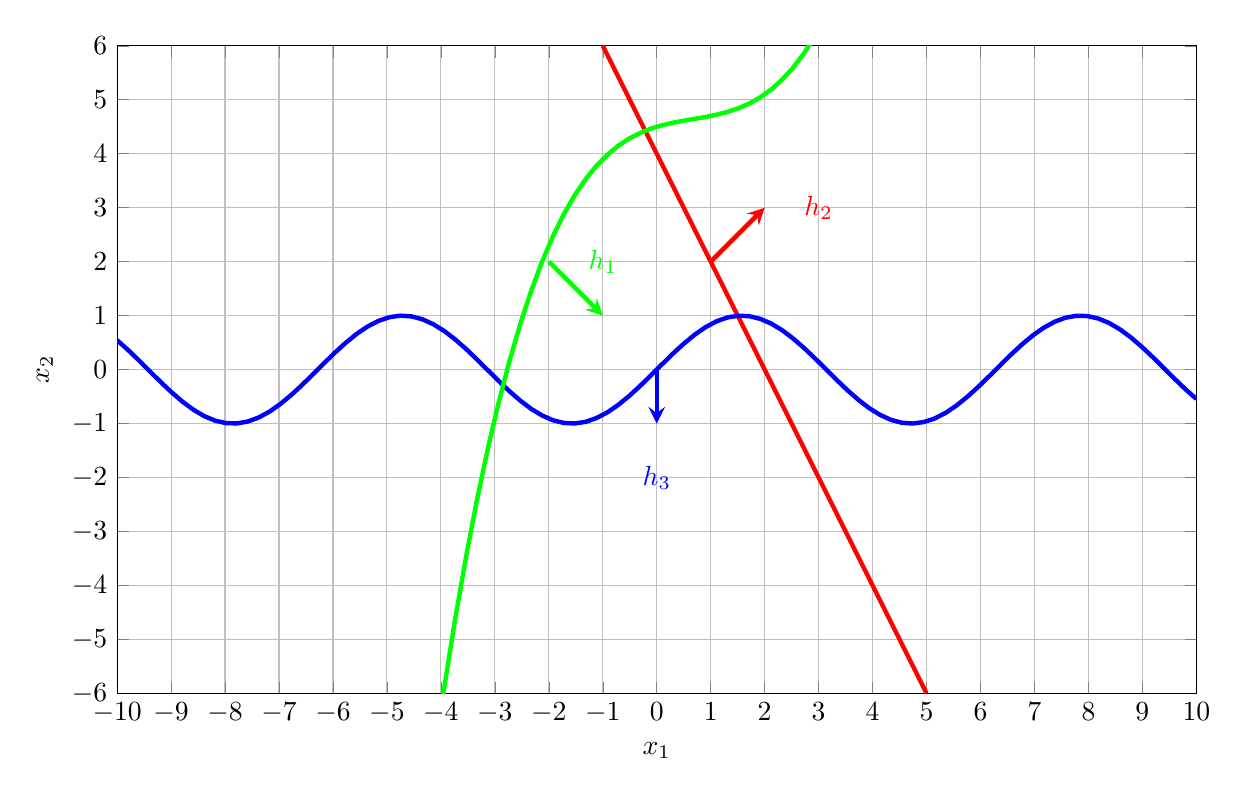
\begin{tikzpicture}
    \begin{axis}[
        scale=2.0, axis equal image,
        xmin=-10, xmax=10, xtick={-10,...,10},
        ymin=-6, ymax=6, ytick={-6,...,6},
        samples=50, grid=major, xlabel=$x_1$, ylabel=$x_2$]

        % Straight line
        \addplot [mark=none, red, ultra thick] coordinates {(5, -6) (-1, 6)};
        \draw [-stealth, red, ultra thick] (1,2)--(2, 3);
        \node at (axis cs:3,3) {\color{red}$h_2$};

        % Sinusoidal function
        \addplot [domain=-10:10, samples=100, blue, ultra thick] {sin(deg(x))};
        \draw [-stealth, blue, ultra thick] (0,0)--(0, -1);
        \node at (axis cs:0,-2) {\color{blue}$h_3$};

        % Third-order polynomial function
        \addplot [domain=-10:10, samples=100, green, ultra thick] {0.1*x^3 - 0.2*x^2 + 0.3*x + 4.5};
        \draw [-stealth, green, ultra thick] (-2,2)--(-1, 1);
        \node at (axis cs:-1,2) {\color{green}$h_1$};
    \end{axis}
    \end{tikzpicture} 
    \end{center}
    \begin{soln}
    
    \begin{center}
    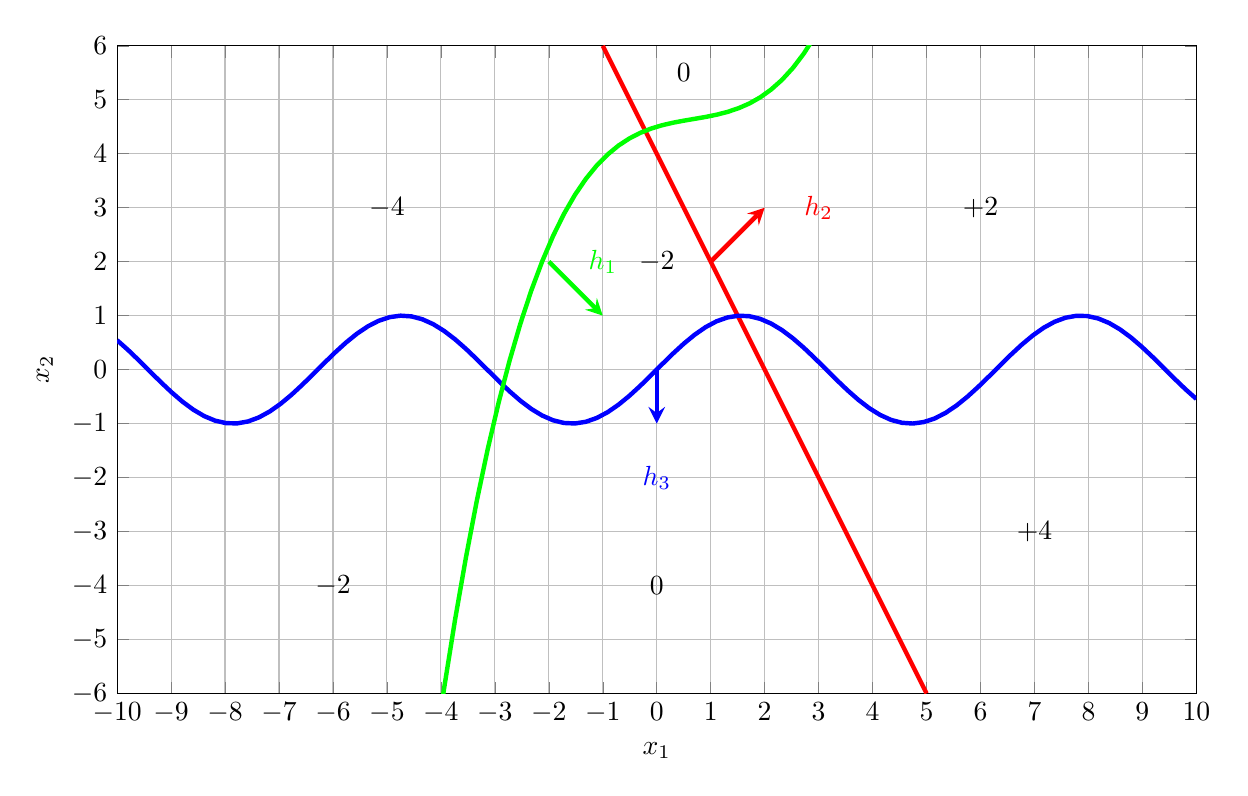
\begin{tikzpicture}
    \begin{axis}[
        scale=2.0, axis equal image,
        xmin=-10, xmax=10, xtick={-10,...,10},
        ymin=-6, ymax=6, ytick={-6,...,6},
        samples=50, grid=major, xlabel=$x_1$, ylabel=$x_2$]

        % Straight line
        \addplot [mark=none, red, ultra thick] coordinates {(5, -6) (-1, 6)};
        \draw [-stealth, red, ultra thick] (1,2)--(2, 3);
        \node at (axis cs:3,3) {\color{red}$h_2$};

        % Sinusoidal function
        \addplot [domain=-10:10, samples=100, blue, ultra thick] {sin(deg(x))};
        \draw [-stealth, blue, ultra thick] (0,0)--(0, -1);
        \node at (axis cs:0,-2) {\color{blue}$h_3$};

        % Third-order polynomial function
        \addplot [domain=-10:10, samples=100, green, ultra thick] {0.1*x^3 - 0.2*x^2 + 0.3*x + 4.5};
        \draw [-stealth, green, ultra thick] (-2,2)--(-1, 1);
        \node at (axis cs:-1,2) {\color{green}$h_1$};

        \node at (axis cs:6,3) {$+2$};
        \node at (axis cs:7,-3) {$+4$};
        \node at (axis cs:0,-4) {$0$};
        \node at (axis cs:0,2) {$-2$};
        \node at (axis cs:0.5,5.5) {$0$};
        \node at (axis cs:-5,3) {$-4$};
        \node at (axis cs:-6,-4) {$-2$};

    \end{axis}
    \end{tikzpicture} 
    \end{center}
    
    \end{soln}
    \begin{qauthor}
    Matt
    \end{qauthor}

\part[2] Given a training dataset $\mathcal{D}$ with $N$ data points, suppose you train a random forest consisting of $B$ decision trees where each tree is trained on $M$ bootstrapped data points (\textbf{Note}: this is a slight deviation from how this material was presented in class in that $M$ is not necessarily equal to $N$). Furthermore, suppose that $K$ features are randomly selected as candidates for each split. 
    
    \textbf{Select all that apply:} Increasing which of the following hyperparameters (while keeping all the others fixed) will tend to \emph{decrease} the variability of the random forest as a whole i.e., make the entire random forest less sensitive to small perturbations to $\mathcal{D}$? 
        {%
        \checkboxchar{$\Box$} \checkedchar{$\blacksquare$} % change checkbox style locally
        \begin{checkboxes}
         \choice $N$
         \choice $B$
         \choice $M$
         \choice $K$
         \choice None of the above
        \end{checkboxes}
        }
        \begin{soln}
            A, B
        \end{soln}
    
    \begin{qauthor}
        Henry
    \end{qauthor}

\end{parts}
